
In this section, we present a detailed description of the methodology used in this thesis. We begin by introducing the Encoder-Decoder architecture, which are crucial components for the VQVAE. We then proceed to describe the VQVAE implementation for timeseries. Finally, we present our modification of the VQVAE, which incorporates the Barlow Twins method to enhance the encoder's ability to learn robust and informative latent representations.

The implementation of the models is based on the paper TimeVQVAE\cite{lee2023masked}. Here they argue for a 2 stage approach. The first stage consists of optimizing the Encoder, Codebook and Decoder to efficiently compress the input into tokens and then reconstruct the input.
This is achieved by minimizing the informational loss obtained by comparing the input $x$ with the reconstructed $\hat{x}$. The next stage consists of training a transformer to approximate the prior.
Stage 1 aligns with our objectives, as we are interested in the latent space generated by the encoder . They base their implementation on a improved approach to VQVAE, designed to extract better high frequency information. We base our implementation on the naive VQVAE as we are interested in the general case for VQVAEs on timeseries.


\section{Encoder}

%The Encoder has the task of compressing the high-dimensional input data into a compact and manageable representation. It is a component of the Variational Auto-Encoder architecture, enabling the compression of input to latent variables.
%The encoded data should capture important characteristics and features from the input data necessary for decompression while also removing unessesary and reduntant information. 
%It operates by using a block like structure, where each block is designed to process the input data sequentially.
The Encoder model, inspired by the fundamental properties of CNNs and the ResNet architecture introduced by He et al.\cite{ResLearn}, is designed to compress the input data into a compact and manageable representation.
Approximating the posterior distribution $q_\phi(z|x)$, the encoder learns to map the input data to a latent space. 
To efficiently approximate the posterior we combine two results: the CNNs ability to learn complex patterns and features within the input data, and the ResNet's ability to train deeper networks. This is achieved by using a block like structure, where each block is designed to process the input data sequentially.

\textbf{Encoder blocks} are the component responsible for giving the model a perceptual view of the input data aswell as downsampling it to a lower dimension. The downsampling is achieved through convolutional layers that strategically reduce the dimensionality of the input, while highlighting important features in non linear activation maps. 
Following the convolutional layer, batch normalization is employed. This technique normalizes the output of the convolution by adjusting and scaling the activations. It allows the network to use higher learning rates, as it reduces the internal covariate shift which in turn makes the learning process more efficient and stable, as described by Ioffe and Szegedy\cite{batchnorm}.

\textbf{Residual blocks} introduce residual or shortcut connections, allowing the encoder to have more layers without sacrifizing efficiency in training. 
These are the building blocks of the original ResNet architecture.

The complete encoder arhitecture is illustrated in figure \ref{fig:Encoder}. The first encoder block is responsible for reducing the dimensionality of the input data. The following encoder blocks sequentially refines the activation maps to include more complex patterns and features.
The number of encoder blocks is determined by a downsampling rate which is determined by the input size and the amount of compression configured for the model. We use the same downsampling rate as done by Lee et al\cite{lee2023masked} in their TimeVQVAE implementation, here they also include four residual blocks.


\begin{figure}[H]
    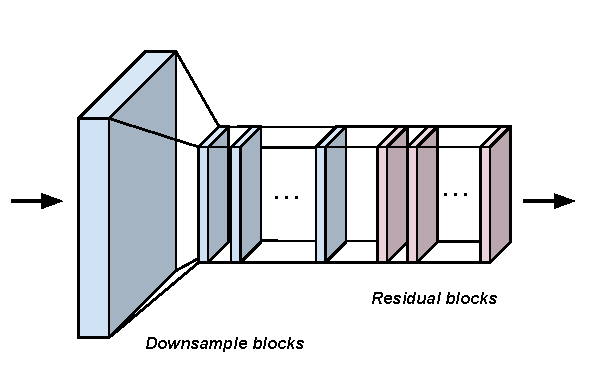
\includegraphics[scale=0.8]{figures/figure-pdf/Encoder.pdf}
    \caption{Illustration of the Encoder architecture.}
    \label{fig:Encoder}
\end{figure}

\section{Decoder}
The Decoder model, also ispired by CNNs and ResNet, is designed to reconstruct the input data from the latent representation. Approximating the likelihood $p_\theta(x|z)$.
Its main function is decompression. It is responsible for the upsampling of the latent representation to a higher dimension, while also refining the feature maps to recover details that were lost during encoding.
Like the encoder the decoder consists of two two types of blocks, decoder blocks and residual blocks.


\textbf{Decoder blocks} are the component responsible for upsampling the latent representation to a higher dimension. This is achieved through the use of transposed convolutional layers, often referred to as deconvolutional layers. These layers effectively reverse the operation of convolution by learning to expand a compressed feature map onto a larger spatial canvas.
The transposed convolutions apply filters in a manner that distributes the encoded feature values over a higher-resolution grid, interpolating additional data points as necessary to achieve the desired output size.
This process not only increases the spatial dimensions but also refines the feature map to recover details that were compressed during encoding.
Following the transpose convolutional layer the upsample block uses batch normalization and ReLu activation function.

The decoder's architecture is characterized by a series residual blocks followed by decoder blocks that progressively restore the data's dimensionality. The number of upsampling blocks is the same as number of downsampling blocks in the encoder. 


\section{VQVAE}
The VQVAE's primary objective is to learn discrete latent representations that can be used to reconstruct the input timeseries data. It is implemented using a Encoder $E$, Decoder $D$ and a vector quantifier.

Prior to the encoder, the input $\mathbf{x}$ (a timeseries) is passed through a Short Time Fourier Transform (STFT), producing $\mathbf{u}$. 

The \textbf{STFT} converts the time-domain signal into a time-frequency representation. This transformation allows the encoder to analyze the signal in both time and frequency domains simultaneously, providing a comprehensive view of the signal's spectral content as it varies over time. 
The encoder thus learns convolutional filters that capture and extract frequency patterns within the input data.
Reversly the Inverse Short Time Fourier Transform (\textbf{ISTFT}) converts the time-frequency representation back to a time-domain representation. 
Both STFT and ISTFT are computational methods grounded in a series of fourier transforms. A key parameter is $n_{\text{fft}}$, dictating the resolution of the frequencies in the transformed domain.
As done in the TimeVQVAE implementation, we set $n_{\text{fft}}$ to be 8.

Next the encoder compresses $\mathbf{u}$ into a continuous latent variable $\mathbf{z}$ followed by a quantization to $\mathbf{z_q}$. Transforming the continous latent space to a discrete latent space. The input is at this state represented as tokens in our codebook.
The tokens or discrete latent variables is then passed through the decoder denoted as $D$, projecting the discrete latent space back into a time-frequency domain, $\hat{\mathbf{u}}$. Where it is then mapped back to a time-domain using ISTFT.
Giving the reconstructed input $\mathbf{\hat{x}}$. This is summerized in the figure \ref{fig:VQVAE}

\begin{center}
\begin{figure}[H]
    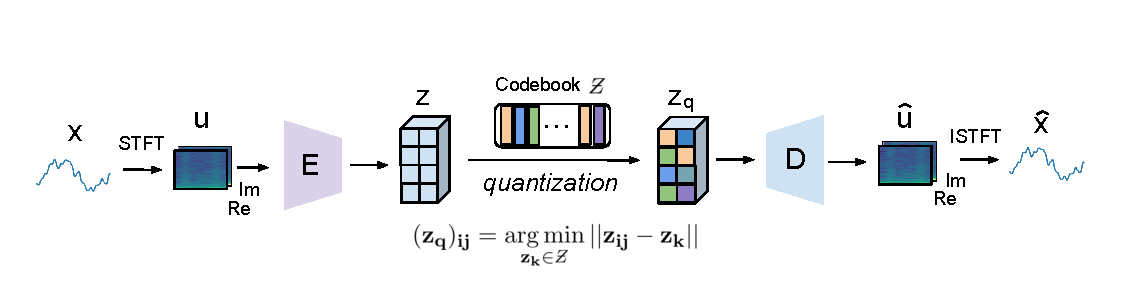
\includegraphics[scale=0.8]{figures/figure-pdf/VQVAE.pdf}
    \caption{ Illustration of the VQVAE. Illustration and implementation inspired by the TimeVQVAE paper\cite{lee2023masked} }
    \label{fig:VQVAE}
\end{figure}
\end{center}

\subsection{Learning}
Learning is achieved through updating the networks parameters through backpropagation. This process requires a formulation of a suitable loss function that reflects the learning objective of the model.

Based on the TimeVQVAE\cite{lee2023masked} paper and the ELBO formulation the total loss for our VQVAE is the sum of two parts. Reconstruction loss, $\mathcal{L}_{\text{recon}}$, and codebook loss, $\mathcal{L}_\text{codebook}$.

\begin{equation}
    \mathcal{L}_{VQVAE} = \mathcal{L}_\text{recon} + \mathcal{L}_\text{codebook}
    \label{eq:VQVAEloss}
\end{equation}

\subsubsection{Reconstruction}
By minimizing the reconstruction loss, $\mathcal{L}_{\text{recon}}$, we align with maximization of $\log p_\theta(x)$ in the ELBO formulation \ref{eq:ELBO}.
We define the reconstruction loss to be:
\begin{equation}
    \mathcal{L}_{\text{recon}} = ||x-\hat{x}||_2^2 + ||u-\hat{u}||_2^2
\end{equation}

This gives us a metric or score on how well the reconstructed timeseries is compared to the input. As the metric acts on both time and time-frequency domain, we ensure that the 
model learns to reconstruct well for both of these domains.

By replacing the norms with MSE we get the implemented reconstruction loss:
\begin{equation}
    \mathcal{L}_{\text{recon}} = MSE(x,\hat{x}) + MSE(u, \hat{u})
    \label{eq:recon}
\end{equation}

\subsubsection{Codebook-learning loss}
The codebook learning loss will ensure that the quantized latent representations, $\mathbf{z_q}$, effectively approximate the continues latent space $\mathbf{z}$, thereby maintaining a structured and meaning full latent representation. 

The codebook-learning loss is defined as
\begin{equation}
    \mathcal{L}_\text{codebook} = ||\text{sg}\left[ E(\text{STFT}(x))\right] - z_q||_2^2 + \beta|| E(\text{STFT}(x)) - \text{sg}\left[ z_q \right]||_2^2
    \label{eq:codebook}
\end{equation}

The first term in the codebook-learning loss,
\begin{equation}
    ||\text{sg}\left[ E(\text{STFT}(x))\right] - z_q||_2^2
\end{equation}
measures the difference between the stop-gradient, $\text{sg}\left[\cdot\right]$, aplied encoded representation and the quantized latent vector $z_q$. This term ensures that the chosen quantized vectors from the codebook is as close as possible to the output of the encoder. By applying the stop gradient operator, we prevent the gradients from backpropagating through the encoder during this part of the loss calculation.
Isolating the calculating to just act on the codebook.

The second term,
\begin{equation}
    \beta|| E(\text{STFT}(x)) - \text{sg}\left[ z_q \right]||_2^2
\end{equation}
encourages the encoder's output to move closer to the quantized vectors. The parameter $\beta$ acts as a balanding factor, controlling the strength. In this implementation we set $\beta$ to be 1 as done in the TimeVQVAE implementation.
By applying the stop gradient on the quantized vector $z_q$, this term focuses on updating the encoder's parameters to produce outputs that are more aligned with the existing
codebook vectors.

Togheter, these two terms ensure that the codebook adapts to the encoded, $z$. Simultaneously, the encoder adapts to the quantized $z_q$. As a result the Encoder is tuned to produce representations that are effectively quantized by the codebook.
As done in the reconstruction loss the norms, $||\cdot||_2^2$, is replaced with MSE in our loss  calculation.
\section{Modifying the VQVAE for Enhanced Self Supervised Learning}
In this section we present our modification of the VQVAE, specifically tailored to leverage the strengths of Self Supervised Learning (SSL).
The primary goal of this modification is to build upon the existing VQVAE architecture, while adapting its encoder to produce more robust and informative latent representations.
To achieve this we propose the integration of the Barlow Twins method with the VQVAE encoder.


\subsection{Modifying the VQVAE encoder}
The proposed modification involves extending the VQVAEs encoder section into a two branch structure. Hence adopting a siamese architecture by augmenting 
the input $\mathbf{x}$ into two views, ($\mathbf{x_A}$, $\mathbf{x_B}$).

The same encoder in both branches then encodes both time-frequency views, ($\mathbf{u_A}$, $\mathbf{u_B}$). Producing two latent variables ($\mathbf{z_A}$, $\mathbf{z_B}$). We continue by calculating the barlow twins loss. First applying a batch normalization, $BN$, then using a projector denoted as $P$ to expand the dimensionality of the latent variables. As done by Zbontar et al in their paper\cite{Barlow}.
After the projection to a higher feature space, the cross correlation matrix, $C$, is calculated followed by the barlow twins loss function, $\mathcal{L}_{BT}$. This is summerized in fig \ref{fig:BTVQVAE}. 
As illustrated, the upper branch is the regular VQVAE and the lower branch is the extension allowing the encoder to process two views.

\begin{figure}[H]
    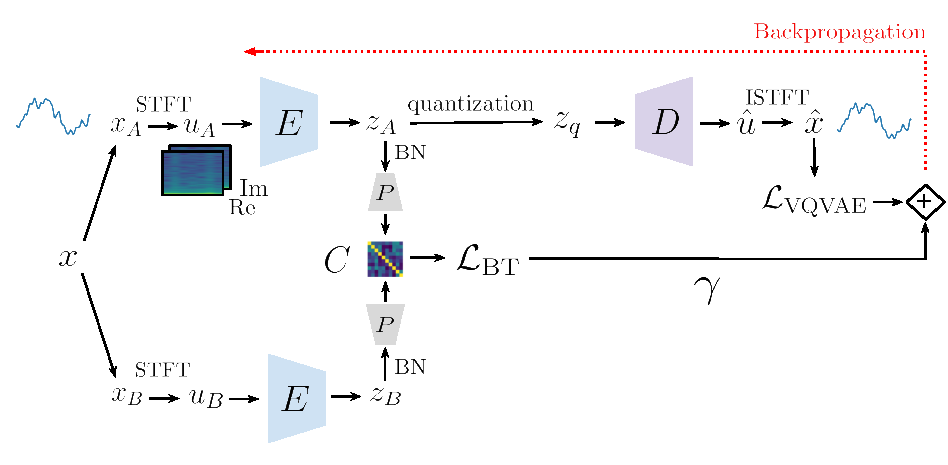
\includegraphics[scale=0.8]{figures/figure-pdf/BarlowTwinsVQVAE.pdf}
    \caption{Illustration of the Barlow Twins modification to VQVAE including the loss function calculation.}
    \label{fig:BTVQVAE}
\end{figure}

\subsubsection{Learning}
The modified VQVAE now has a additional SSL objective. As done by Bardes et al in their paper VICReg\cite{VICReg} we scale the barlow twins loss by the projected feature dimension, $d$, visualized in fig \ref{fig:Barlow}. Our Barlow Twins loss is extended as follows:

\begin{equation}
\mathcal{L}_{BT}(\mathbf{z_1}, \mathbf{z_2}) =\frac{1}{d} \left[ \sum_i (1 - C_{ii})^2 + \lambda \sum_i \sum_{j \neq i} C_{ij}^2\right]
\end{equation}

In the original barlow twins paper\cite{Barlow} they found that a low valued $\lambda$ equal to $0.005$ gave the optimal balance between invariance and redundancy reduction. They also found that the dimensionality of the projector had a substantial effect on the 
efficiency of the barlow twins loss calculation. A higher dimensionality gave better results. Based on this find, we expand the encoded dimension to $d=4096$ as done by Lee et al\cite{SSLs}. 
The projector architecture consist of a max pooling layer followed by a fully connected neural

The total loss function, $\mathcal{L}_{\text{BT-VQVAE}}$, of our modified VQVAE becomes:

\begin{equation}
    \mathcal{L}_{\text{BT-VQVAE}} = \mathcal{L}_{\text{VQVAE}} + \gamma \cdot \mathcal{L}_\text{BT}
    \label{eq:BTVQVAEloss}
\end{equation}

The loss calculation is visualized in fig \ref{fig:BTVQVAE}. The parameter $\gamma$ determines the weight of the barlow twins loss in the calculation. The $\mathcal{L}_{VQVAE}$ is calculated as done in eq \ref{eq:VQVAEloss} using the upper branch reconstruction and codebook.

\subsection{Augmentation Techniques}
The augmentation techniques employed in this implementation, inspired by the paper by Wen et al\cite{augs} and the paper by Lee and Aune\cite{SSLs}, are categorized into time domain augmentations and time-frequency domain augmentations. 
A good augmentation should preserve overall schemantics of the timeseries during the transformation. 

\subsubsection*{Time Domain Augmentations}
These techniques manipulate the time series data directly in the time domain. A summerization of the implemented techniques are:
\begin{itemize}
    \item \textbf{Flipping}: Reversing the sequence of the time series, simulating time-reversed scenarios.
    \item \textbf{Jittering}: Adding Gaussian noise to the time series, introducing random variations akin to sensor noise or measurement errors.
    \item \textbf{Amplitude Resizing}: Adjusting the amplitude of the time series, simulating variations in signal strength.
    \item \textbf{Adding Slope}: Incorporating a linear trend, emulating gradual shifts or drifts in the data.
\end{itemize}

\subsubsection*{Time-Frequency Domain Augmentations}
These techniques operate on the time-frequency representation of the time series, offering a different perspective for augmentation:

\textbf{STFT Augmentation}: The most comprehensive technique in this implementation is the STFT (Short Time Fourier Transform) augmentation. It involves transforming the time series into the frequency domain using STFT, modifying the phase components using noise, and then reconstructing the time series. This process is particularly effective in introducing complex and subtle variations that are not easily achievable through direct time domain manipulations.

\begin{figure}
    \centering
    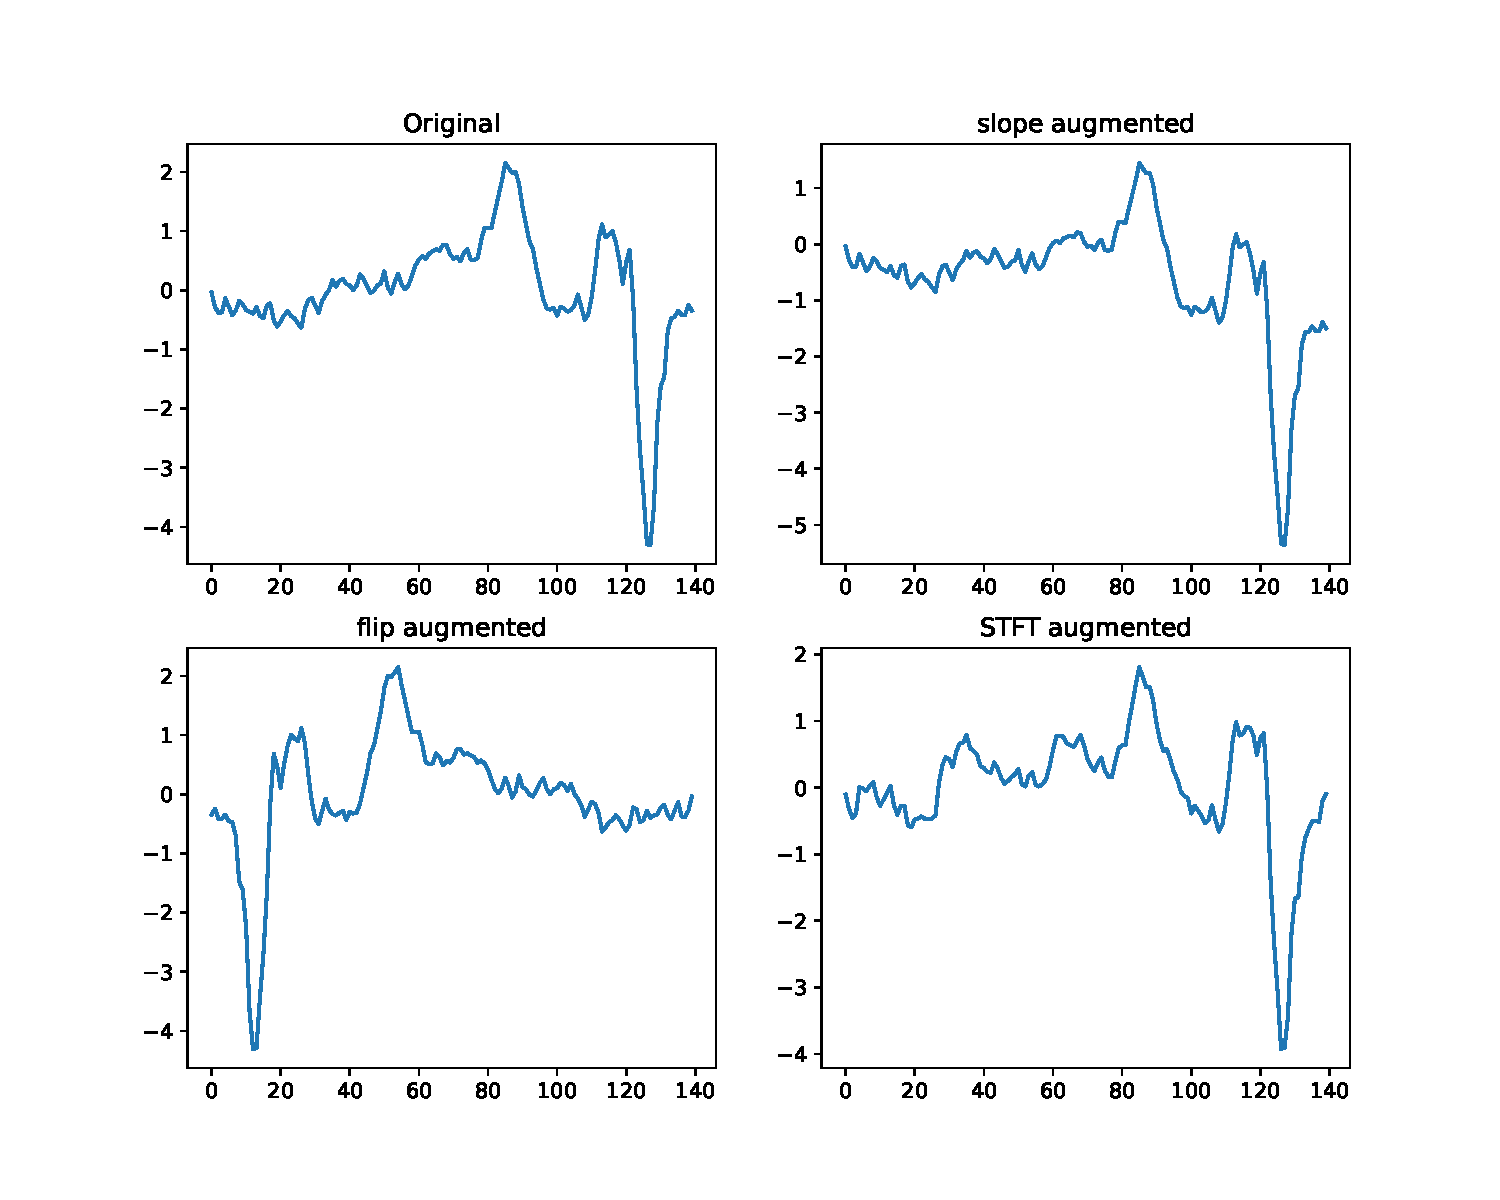
\includegraphics[width=\textwidth]{figures/figure-pdf/Augmentations.pdf}
    \caption{Visualization of the flip, slope and STFT augmentation aplied on a timeseries. }
\end{figure}
